\subsubsection{Cálculos}

\begin{frame}
\frametitle{Cálculo da máxima deflexão}
    $$Y_{max} = \frac{F \cdot L^{3}}{48 \cdot E \cdot I}$$
    \begin{figure}
        \centering
        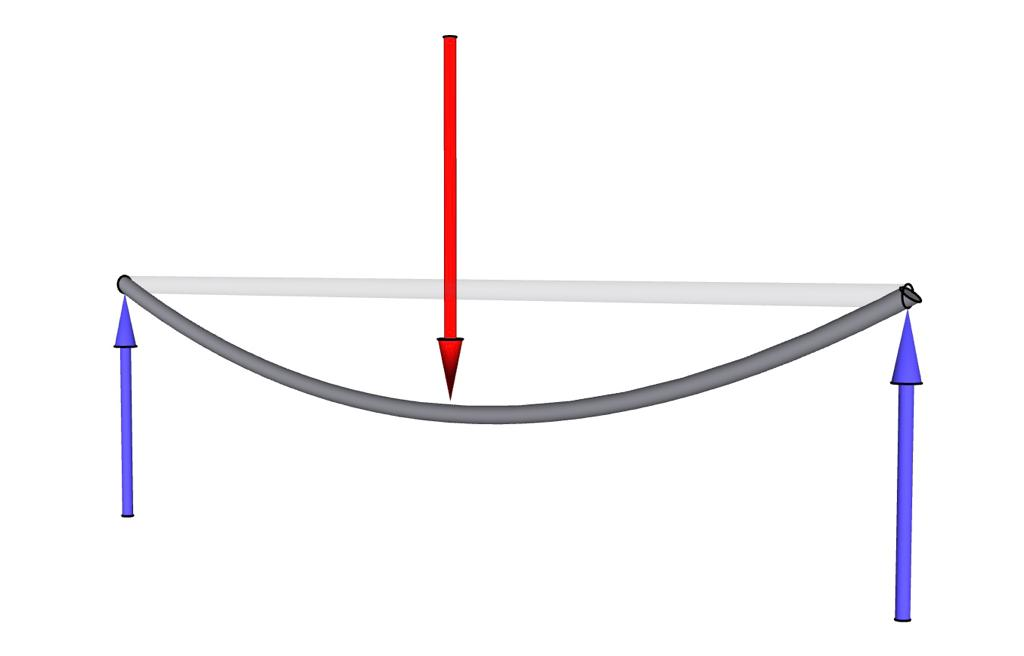
\includegraphics[scale = 0.1]{figuras/diagramcorpolivre}
        \caption{Diagrama de corpo livre da haste}
    \end{figure}
\end{frame}

\begin{frame}
\frametitle{Cálculo da força máxima suportada pelo fuso}
    \begin{columns}
        \begin{column}{0.7\textwidth}
            $$T = \frac{F \cdot d_{m}}{2} \cdot (\frac{L_{a} + \pi \cdot f \cdot d_{m}}{\pi \cdot d_{m} - f \cdot L_{a}}) + \frac{F \cdot f_{c} \cdot d_{c}}{2}$$
        \end{column}
        \begin{column}{0.3\textwidth}
            \begin{figure}
                \centering
                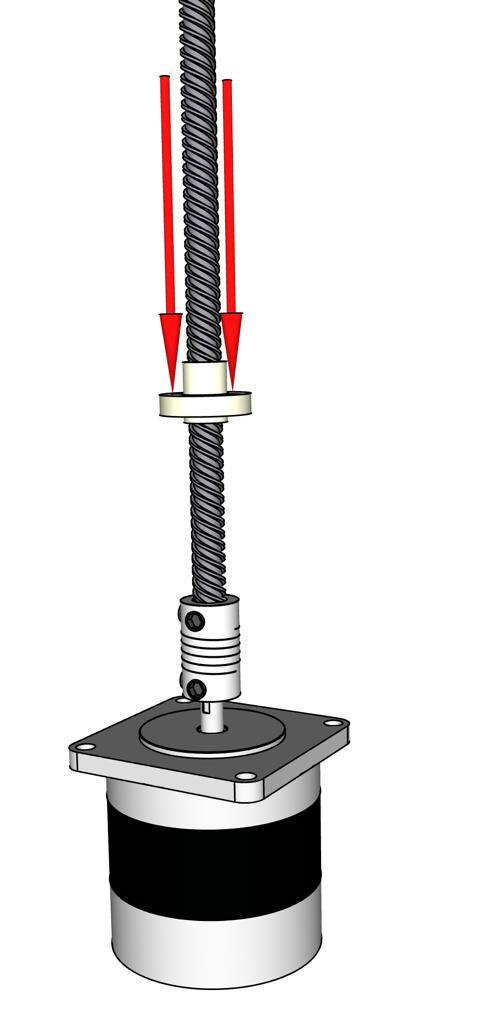
\includegraphics[scale = 0.15]{figuras/esqforcafuso}
            \end{figure}
        \end{column}
    \end{columns}
\end{frame}

\begin{frame}
\frametitle{Cálculo da força máxima suportada pelo fuso}
    \begin{columns}
        \begin{column}{0.7\textwidth}
            Tensão de flexão da raiz da rosca:
            $$\sigma_{raiz} = \frac{6 \cdot (0,38 \cdot F)}{\pi \cdot d_{r} \cdot n_{t} \cdot P}$$
            Tensão de cisalhamento máximo:
            $$\sigma_{2}, \sigma_{3} = \frac{\sigma_{x} + \sigma_{y}}{2} \pm \sqrt{(\frac{\sigma_{x} - \sigma_{y}}{2})^2 + \tau_{xy}^{2}}$$
            Tensão Máxima:
            $$\sigma_{1-3} = \frac{\sigma_{1} - \sigma{3}}{2}$$
        \end{column}
        \begin{column}{0.3\textwidth}
            \begin{figure}
                \centering
                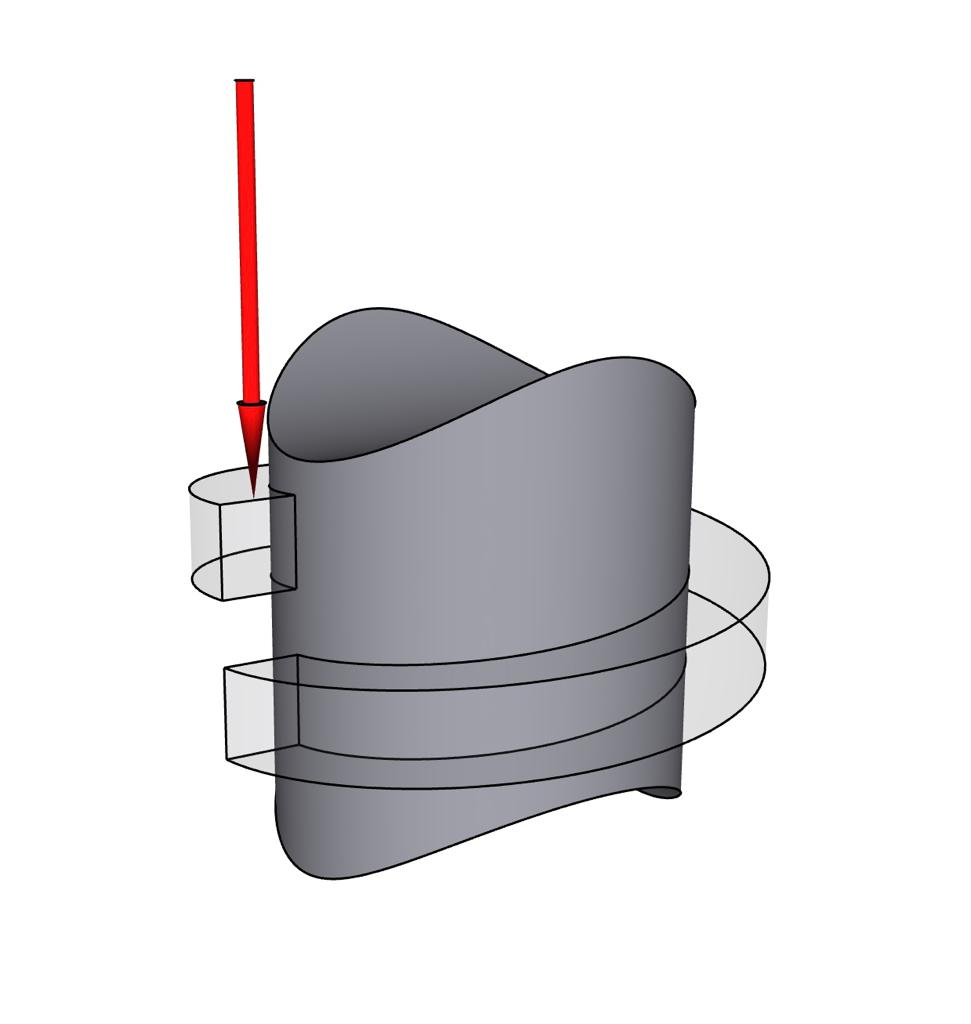
\includegraphics[scale = 0.09]{figuras/forcadente}
            \end{figure}
        \end{column}
    \end{columns}
\end{frame}
    